\documentclass[10pt]{beamer}
\usepackage{fontspec}
\usepackage{graphicx}
\usepackage{parskip}
\usepackage{alltt}
\usepackage{tabularx}
\usepackage{setspace}
\usepackage{/home/james/src/latex_packages/pgfgantt/pgfgantt}
\usepackage{adjustbox}
\usepackage{caption}
\usepackage{subcaption}

\setbeamercolor{title}{fg=black}
\setbeamercolor{frametitle}{fg=black}
\setbeamercolor{sectiontitle}{fg=black}
\setbeamercolor{local structure}{fg=black}
\setbeamertemplate{itemize items}[circle]
\setbeamertemplate{navigation symbols}{}
\usefonttheme{serif}
\setmainfont{Noto Sans}


\title{\textbf{Plan3}}
\author{James Engleback}

\begin{document}

\begin{frame}
\maketitle
\end{frame}

\begin{frame}
	\begin{spacing}{0.00}
	\tiny\tableofcontents
	\end{spacing}
\end{frame}

\section{Dependency Graphs}
\begin{frame}
	\frametitle{\textbf{Dependency Graphs}}

	\begin{figure}
	\begin{subfigure}{0.49\linewidth} 
	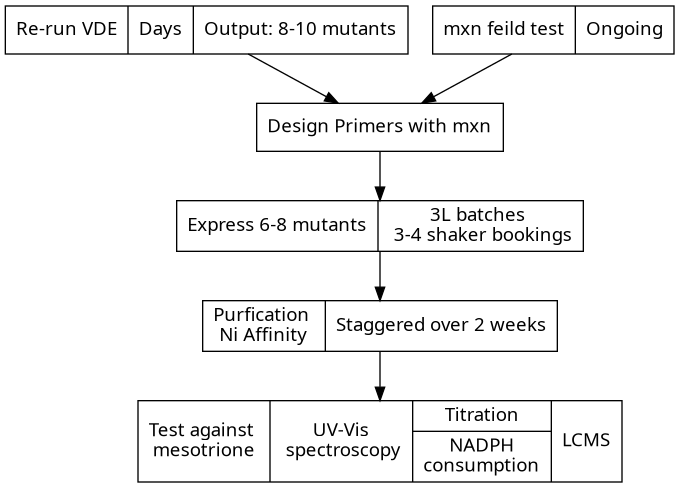
\includegraphics[width=\textwidth]{figs/evoG.png}
		\caption{\label{evoG} - dependency graph of the remainder of the virtual directed evolution project}
	\end{subfigure}
	\begin{subfigure}{0.49\linewidth} 
	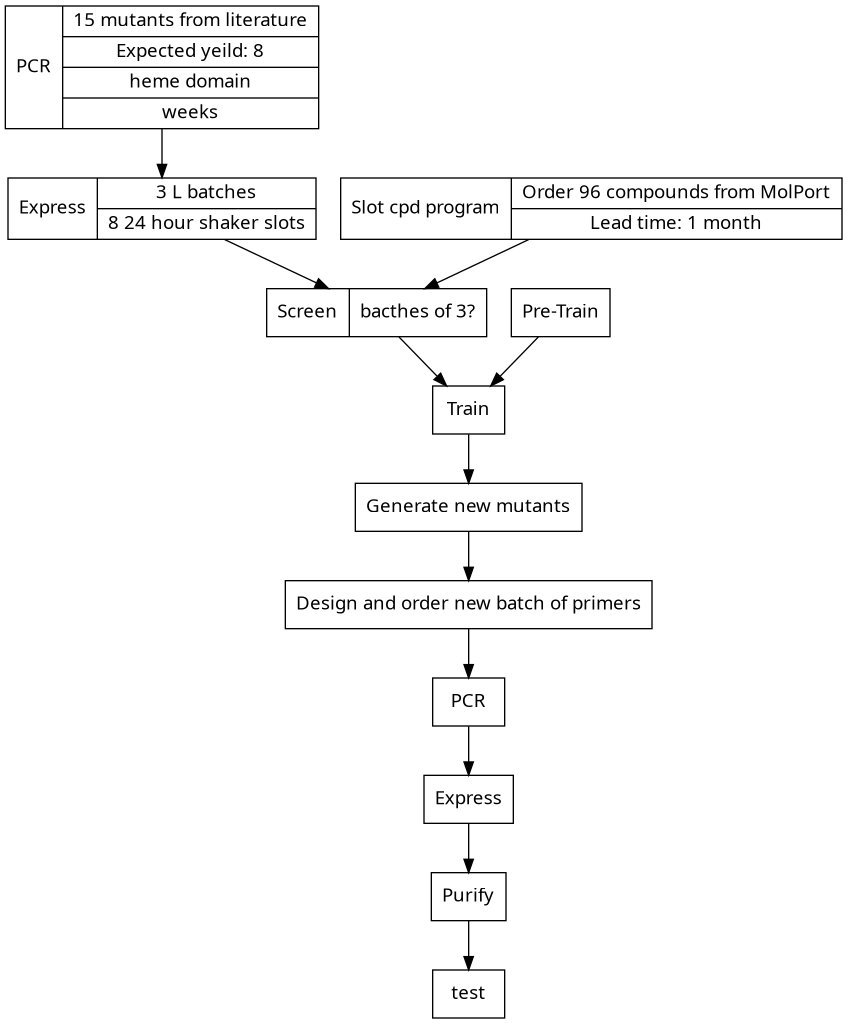
\includegraphics[width=\textwidth]{figs/rioG.png}
		\caption{\label{rioG} - dependency graph for the remainder of the AI-based design project}
	\end{subfigure}
	\end{figure}
\end{frame}

\section{Schedule}
\begin{frame}
\begin{adjustbox}{max totalsize={\textwidth}{.8\textheight},center}

	\fontsize{4pt}{4pt}
	\frametitle{\textbf{Schedule}}
\begin{ganttchart}[time slot format=isodate, y unit chart = 5mm, x unit = 1.8mm, vgrid, hgrid]{2021-05-17}{2021-09-18}{week}
	\gantttitlecalendar{month = name, week=3} \\
	\ganttbar{\textbf{VDE:} VDE}{2021-05-17}{2021-05-25} \\
	\ganttbar{\textbf{VDE:} Primer Design}{2021-05-25}{2021-05-26} \\
	\ganttbar{\textbf{VDE:} Primer Shipping}{2021-05-26}{2021-06-03} \\
	\ganttbar{\textbf{VDE:} DNA work}{2021-06-03}{2021-06-17} \\
	\ganttbar{\textbf{VDE:} Expression}{2021-06-11}{2021-06-25} \\
	\ganttbar{\textbf{VDE:} Purification}{2021-06-18}{2021-07-03} \\
	\ganttbar{\textbf{VDE:} Validation}{2021-07-03}{2021-07-10} \\
	\\
	%%%%%%%%%%%
	\ganttbar{\textbf{AI: }DNA Work}{2021-05-17}{2021-06-09} \\
	\ganttbar{\textbf{AI: }Compound Selection}{2021-05-17}{2021-05-26} \\
	\ganttbar{\textbf{AI: }Expression}{2021-05-26}{2021-06-25} \\
	\ganttbar{\textbf{AI: }Purification}{2021-06-18}{2021-07-03} \\
	\ganttbar{\textbf{AI: }Screening}{2021-06-20}{2021-07-17} \\
	\ganttbar{\textbf{AI: }Pre-Training}{2021-07-03}{2021-07-17} \\
	\ganttbar{\textbf{AI: }Training}{2021-07-17}{2021-07-24} \\
	\ganttbar{\textbf{AI: }Mutant Generation}{2021-07-24}{2021-07-31} \\
	\ganttbar{\textbf{AI: }Primer Design}{2021-07-31}{2021-08-02} \\
	\ganttbar{\textbf{AI: }DNA work}{2021-08-09}{2021-08-21} \\
	\ganttbar{\textbf{AI: }Expression}{2021-08-21}{2021-09-04} \\
	\ganttbar{\textbf{AI: }Purification}{2021-08-26}{2021-09-08} \\
	\ganttbar{\textbf{AI: }Validation}{2021-09-03}{2021-09-12} \\
\end{ganttchart}
\end{adjustbox}
\end{frame}

\begin{frame}
	\frametitle{\textbf{Outstanding Issues, Questions and Loose Ends}}
	\begin{itemize}
		\item \texttt{enz} benchmark
		\item Site directed mutagenesis and \texttt{mxn}
		\item plate assay discussion
		\item compound library
		\item out of hours access
	\end{itemize}
\end{frame}

\section{DNA Work}
\begin{frame}
	\frametitle{\textbf{DNA Work}}
	current limiting factor \\
	got colonies - we'll see \\
	\begin{figure}
		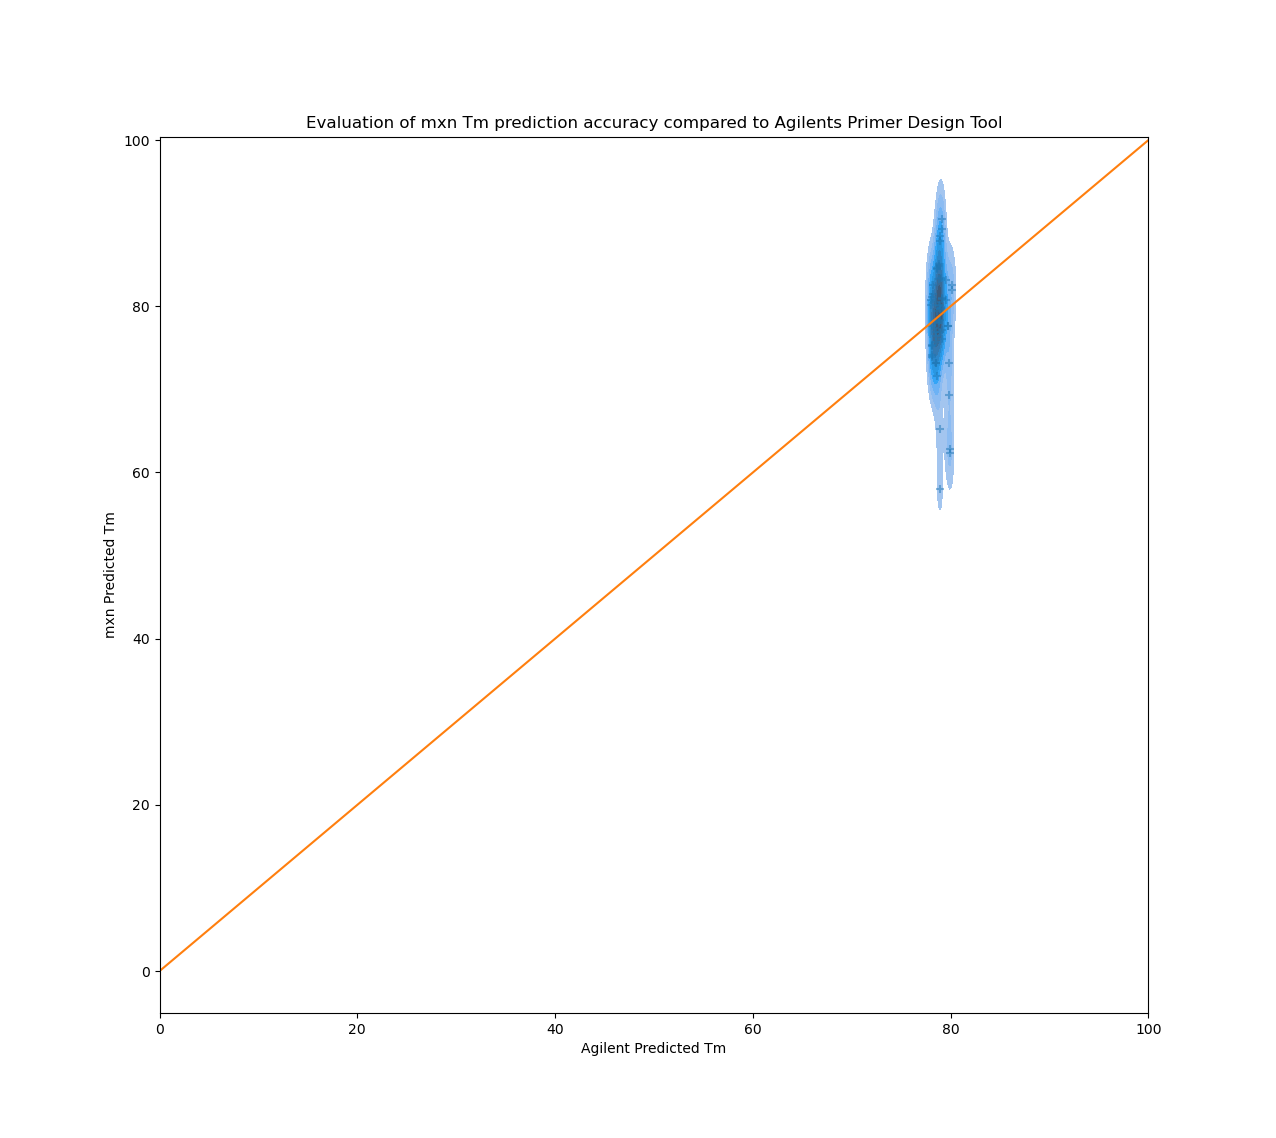
\includegraphics[width=0.6\textwidth]{figs/mxn.png}
		\caption{\label{mxn} oh jeez}
	\end{figure}
\end{frame}

\begin{frame}
	\frametitle{\textbf{DNA Work}}
	\textbf{ongoing and to do} \\ 
	\textbf{AI-based design:} recreating 15 mutants from literature - ongoing, we have colonies!
	\par
	\textbf{Virtual Directed Evolution (to do):} Create final set
\end{frame}

\section{Plate Assay}
\begin{frame}
	\frametitle{\textbf{Plate Assay }}
	\begin{figure}
	\begin{subfigure}{0.49\linewidth} 
	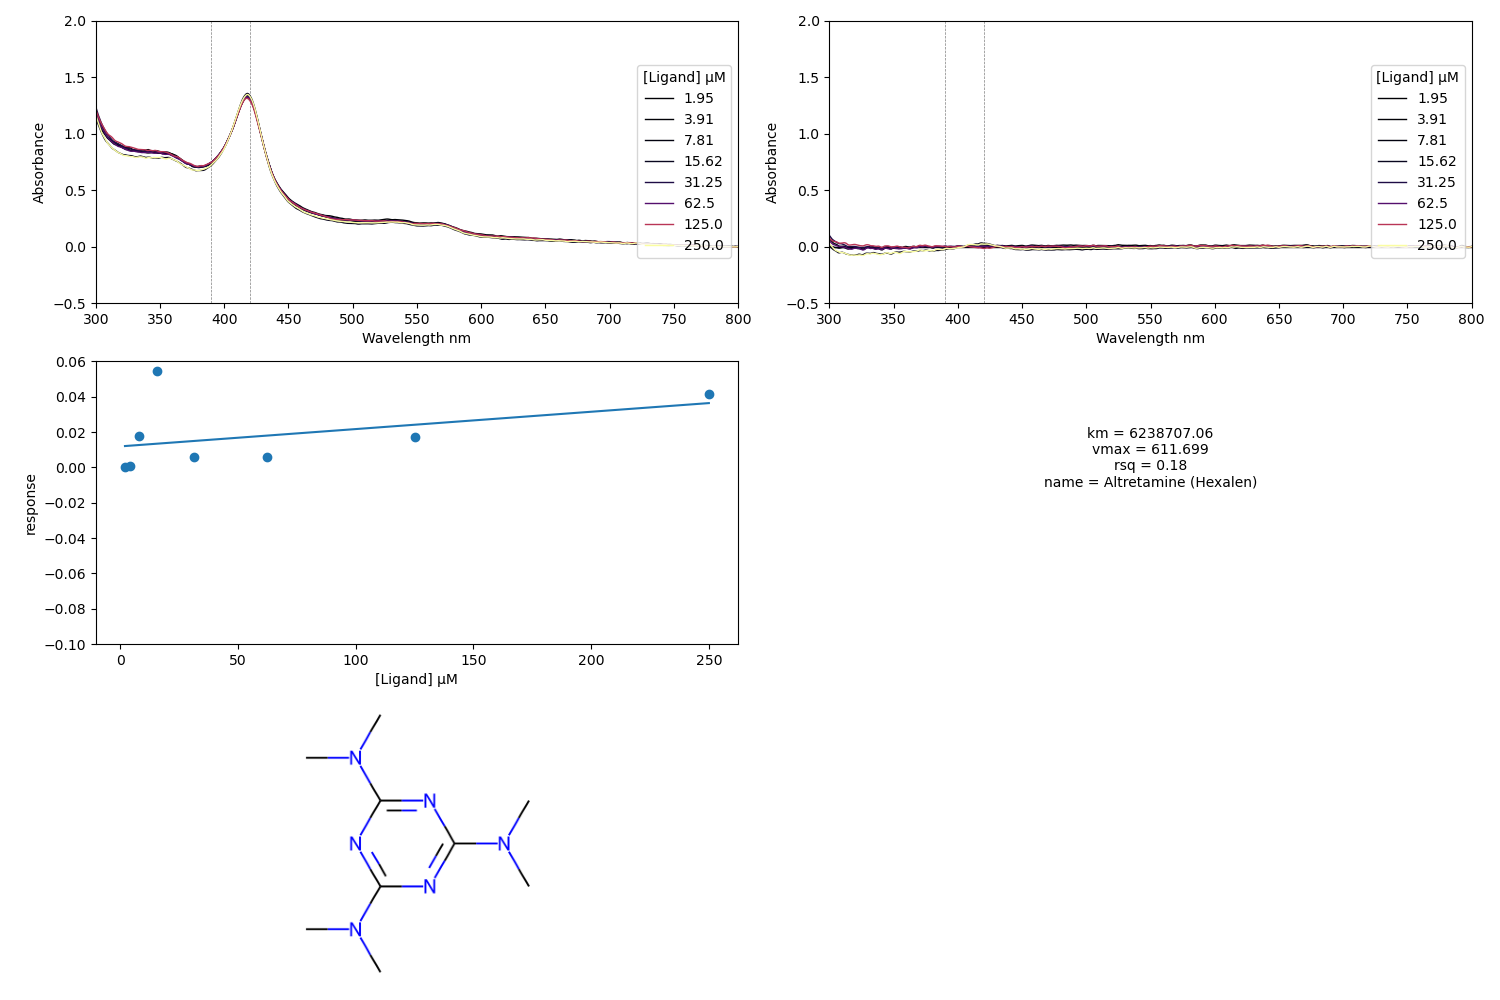
\includegraphics[width=\textwidth]{figs/Altretamine(Hexalen).png}
	\end{subfigure}
	\begin{subfigure}{0.49\linewidth} 
	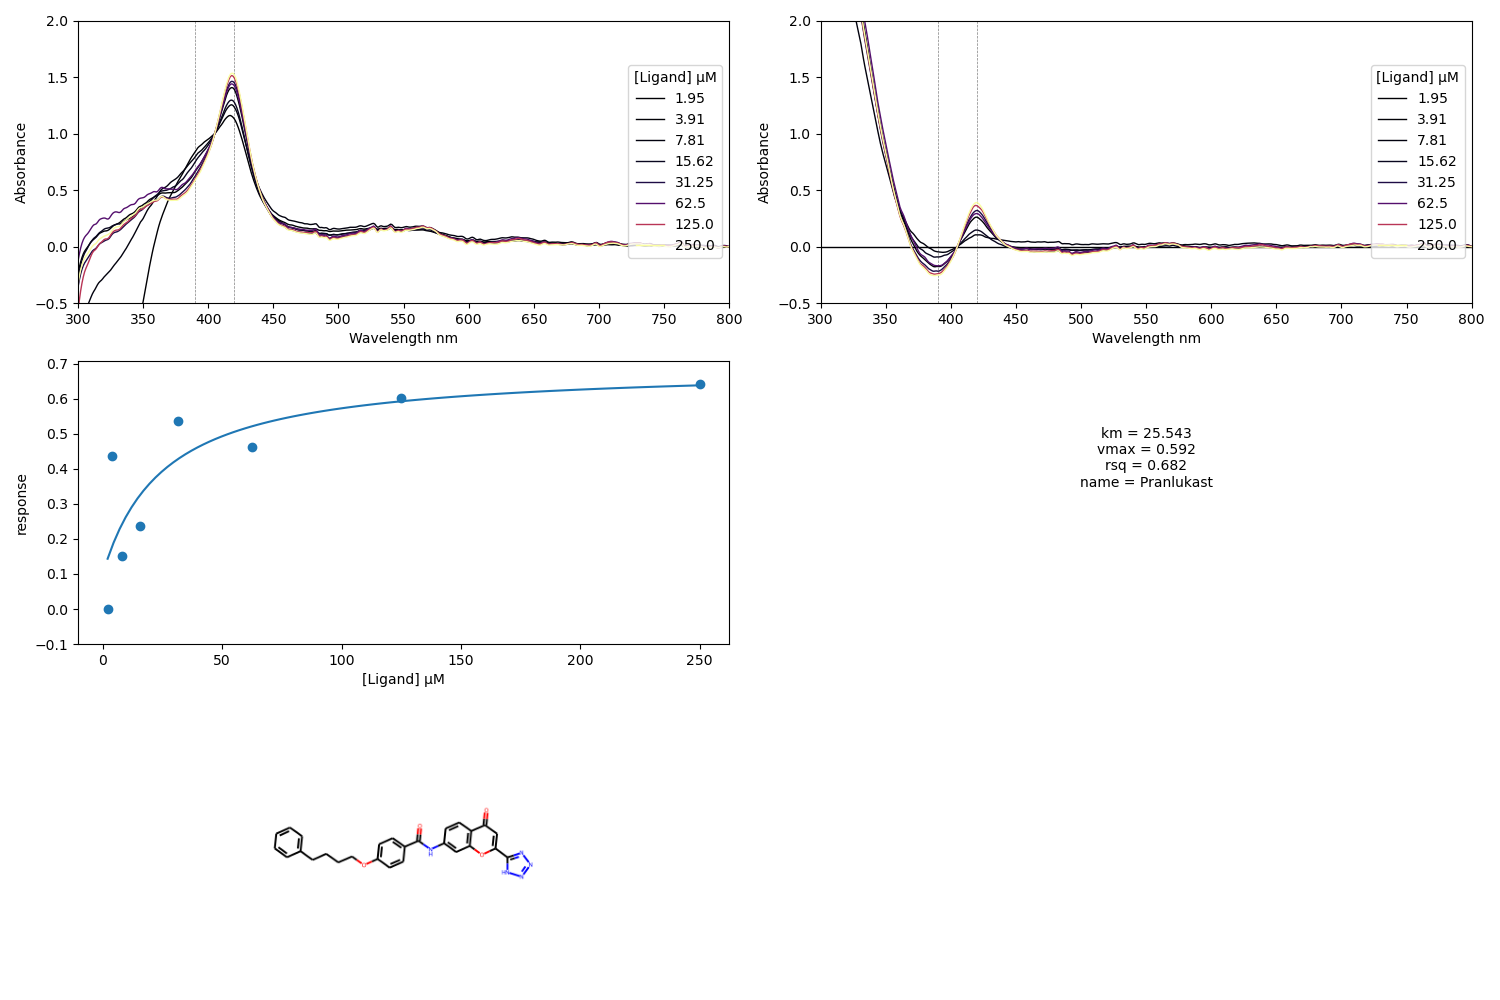
\includegraphics[width=\textwidth]{figs/Pranlukast.png}
	\end{subfigure}
	\begin{subfigure}{0.49\linewidth} 
	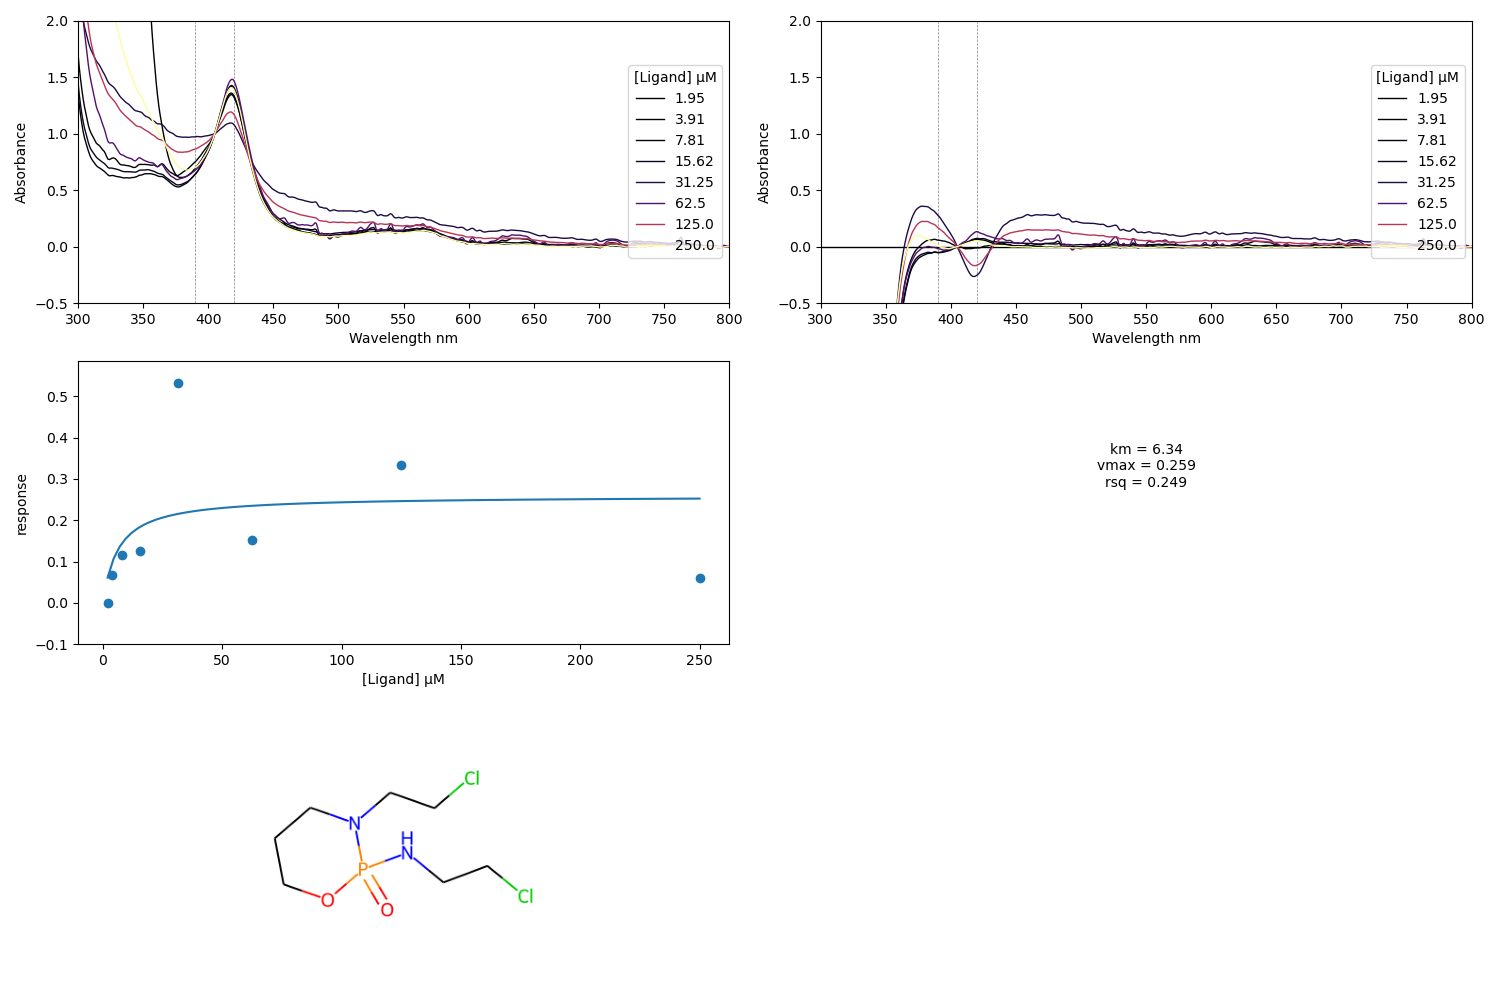
\includegraphics[width=\textwidth]{figs/15.png}
	\end{subfigure}
		\caption{\label{ok-ones} Some ok ones}
	\end{figure}
\end{frame}

\begin{frame}
	\frametitle{\textbf{Plate Assay }}
	\begin{figure}
	\begin{subfigure}{0.49\linewidth} 
	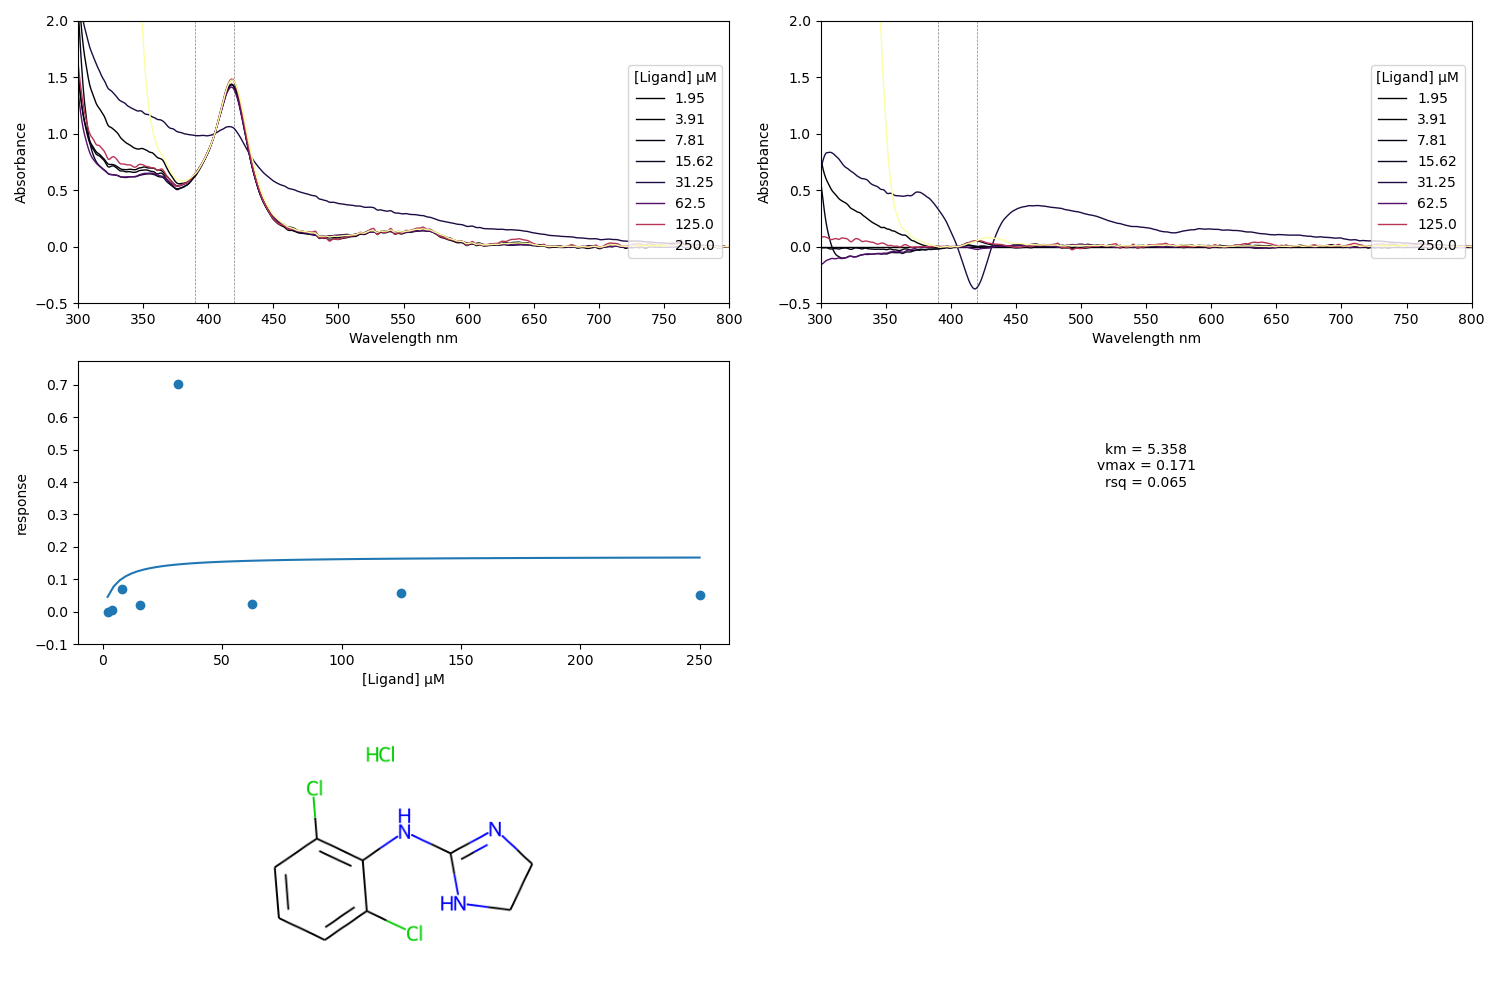
\includegraphics[width=\textwidth]{figs/32.png}
	\end{subfigure}
	\begin{subfigure}{0.49\linewidth} 
	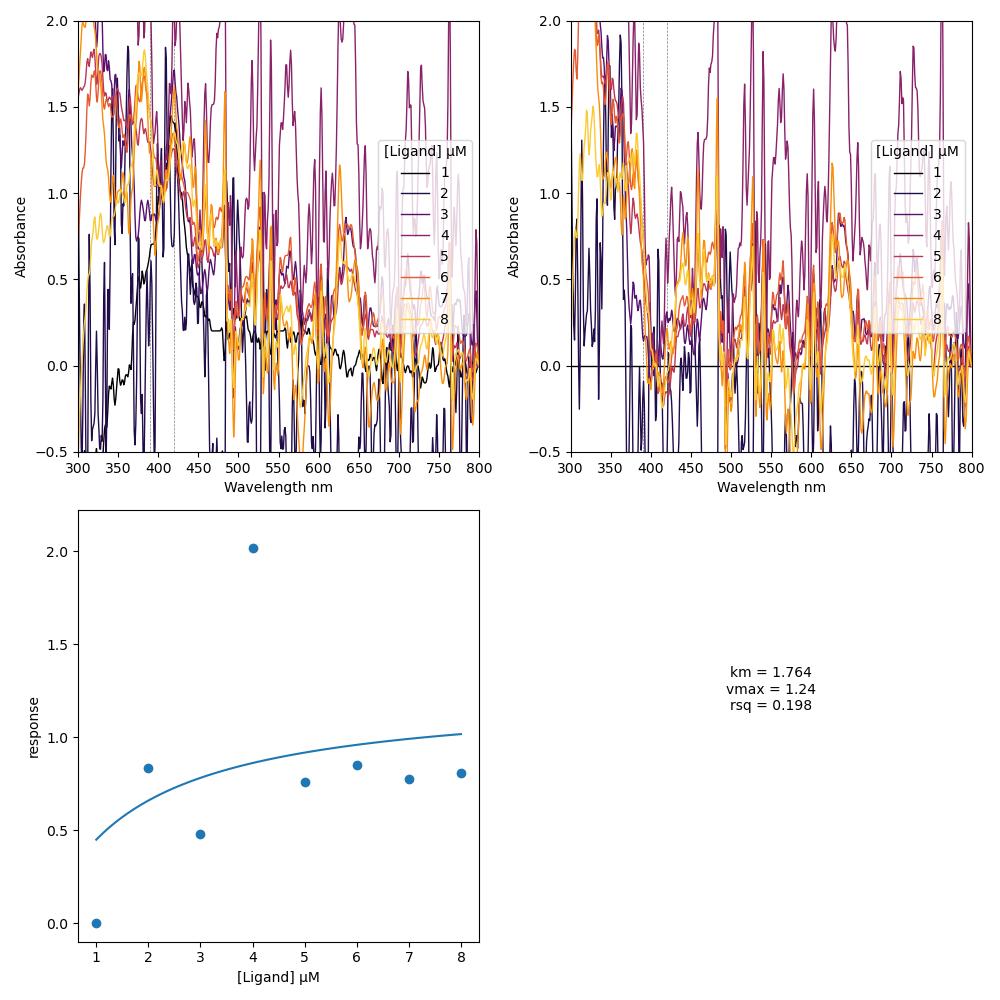
\includegraphics[width=\textwidth]{figs/bad-trace.png}
	\end{subfigure}
		\caption{\label{bad-ones} some bad ones}
	\end{figure}
\end{frame}

\begin{frame}
	\frametitle{\textbf{Plate Assay }}
	\textbf{Issues} \\
	scattering - probably frozen DMSO \\
	\textbf{todo}\\
	have another go without using the fridge
\end{frame}


\section{Compounds}
\begin{frame}
	\frametitle{\textbf{Compounds!}}
	FDA
\end{frame}
\end{document}
